% !TeX program = pdflatex
% !TeX root = FCShowReferenceCard.tex

\documentclass[../FeynCalcManual.tex]{subfiles}
\begin{document}
\hypertarget{fcshowreferencecard}{
\section{FCShowReferenceCard}\label{fcshowreferencecard}\index{FCShowReferenceCard}}

\texttt{FCShowReferenceCard[\allowbreak{}\{\allowbreak{}name\}]} shows
the reference card that corresponds to \texttt{"name"}. Reference cards
are stored in Tables/ReferenceCards inside the FeynCalc main directory.
\texttt{FCShowReferenceCard[\allowbreak{}]} lists available reference
cards.

\subsection{See also}

\hyperlink{toc}{Overview}

\subsection{Examples}

\begin{Shaded}
\begin{Highlighting}[]
\NormalTok{FCShowReferenceCard}\OperatorTok{[]}
\end{Highlighting}
\end{Shaded}

\begin{dmath*}\breakingcomma
\left(
\begin{array}{c}
 \;\text{FeynArts} \\
\end{array}
\right)
\end{dmath*}

\begin{Shaded}
\begin{Highlighting}[]
\NormalTok{FCShowReferenceCard}\OperatorTok{[\{}\StringTok{"FeynArts"}\OperatorTok{\}]}
\end{Highlighting}
\end{Shaded}

\begin{figure}[!ht]
\centering
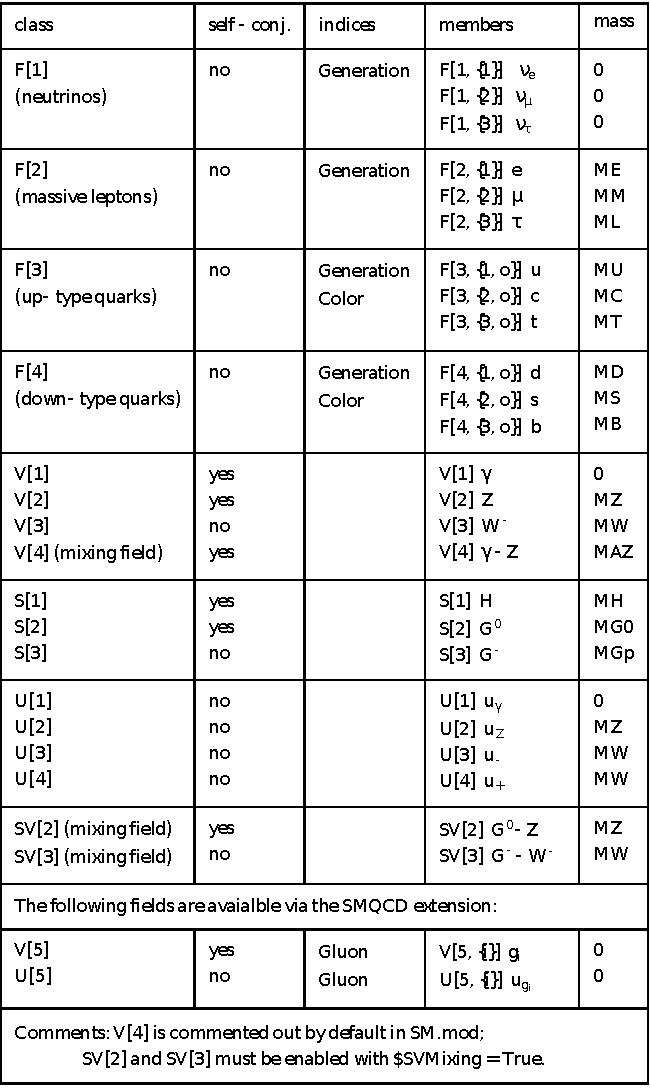
\includegraphics[width=0.6\linewidth]{img/1srqg00tuwkkz.pdf}
\end{figure}
\end{document}
